\chapter{METODOLOGIA E IMPLEMENTAÇÃO DO AMBIENTE DE TESTES}

Este capítulo detalha o artefato experimental (API REST, NGINX, Docker e roteiros de coleta) projetado para responder às questões de pesquisa do Capítulo 1, com proxy reverso como estratégia de integração diante da ausência de suporte nativo estável a HTTP/3 no Node.js (KOCH; FALOWO; ELROD, 2024).

Trata-se de um estudo de caso experimental com abordagem quantitativa: constrói-se um artefato de software reprodutível, define-se uma matriz de cenários controlados e coletam-se métricas de desempenho comparáveis entre HTTP/1.1, HTTP/2 e HTTP/3.

\section{Descrição geral do sistema}

A API REST em Node.js foi construída para avaliações de desempenho, com ambiente controlado que permite comparar HTTP/1.1, HTTP/2 e HTTP/3 sob o mesmo contrato de rotas. A estratégia central consiste em expor HTTP/3 na borda por meio de um proxy reverso NGINX, enquanto o \textit{backend} permanece em HTTP/1.1, em linha com estudos que comparam HTTP/3 e HTTP/2 com integração de proxy (MUÑOZ et al., 2025; TRIPATHI; MIRAZ; JOSHI, 2023). O cliente acessa a API por três caminhos de transporte:

\begin{enumerate}[label=\alph*)]
\item HTTP/1.1 (baseline) - requisições diretas a http://localhost:3000, sem inter-mediário;
\item HTTP/2 via proxy - requisições a https://localhost:8443, com terminação TLS e ALPN HTTP/2 no NGINX;
\item HTTP/3 via proxy - requisições a https://localhost:8443, com terminação QUIC/UDP no NGINX.
\end{enumerate}

Em todos os caminhos, o contrato REST da API - rotas, métodos e formatos de resposta - permanece idêntico; apenas a camada de transporte e a topologia (direto versus via NGINX) variam, conforme a Seção 2.6. Isso isola diferenças de implementação da aplicação, mas não elimina a assimetria estrutural entre HTTP/1.1 direto e os protocolos terminados no proxy - limitação tratada na análise dos resultados (TRIPATHI; MIRAZ; JOSHI, 2023; PERNA et al., 2022).

O ambiente experimental foi delimitado a um cenário controlado de laboratório, sem \textit{frontend}, sem implantação em produção em larga escala e sem modificação do núcleo do Node.js, conforme a Seção 1.9. As questões de pesquisa orientam o desenho do artefato da seguinte forma:

\begin{enumerate}[label=\alph*)]
\item viabilidade (QP1) - verificar se HTTP/3 pode ser utilizado com Node.js por meio de proxy reverso;
\item desafios técnicos (QP2) - documentar configuração, observabilidade e trade-offs opera-cionais (Seção 4.2.4);
\item desempenho comparativo (QP3) - medir latência, tempo de resposta, TTFB, throughput e requisições por segundo (Seção 2.8);
\item estratégias de integração (QP4) - tornar reprodutível a arquitetura proxy + API REST.
\end{enumerate}

A Figura 2 resume os três caminhos de acesso e o papel do proxy reverso na terminação de HTTP/2 e HTTP/3.

\begin{figure}[htbp]
\centering
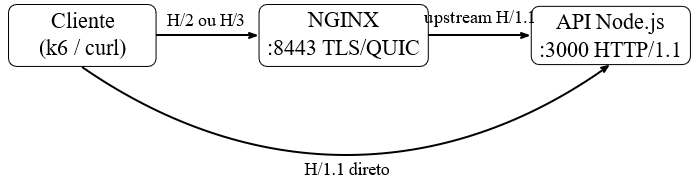
\includegraphics[width=0.92\textwidth]{assets/figuras/image4.png}
\caption{Arquitetura experimental: baseline HTTP/1.1 e caminhos HTTP/2/HTTP/3 via NGINX}
\fonte{Fonte: elaborado pelo autor.}
\end{figure}

O código-fonte do artefato está disponível no repositório \url{https://github.com/mendeslian/QUICBench-Node}, permitindo a reprodução do ambiente descrito neste capítulo.

\section{Infraestrutura e ferramentas}

\subsection{Ambiente de execução}

O ambiente de execução foi construído sobre Node.js (versão $\geq$ 18), executando a API em TypeScript com o \textit{framework Express} 5. A orquestração do \textit{proxy} HTTP/3 utiliza \textit{Docker} e \textit{Docker }\textit{Compose}. O artefato prevê dois modos de implantação, distintos em topologia, mas com o mesmo contrato REST e os mesmos caminhos de protocolo expostos ao cliente:

\begin{enumerate}[label=\alph*)]
\item modo desenvolvimento e validação (host): o contêiner NGINX (docker-compose.yml, infra/nginx/nginx.conf) termina HTTP/2 e HTTP/3 na porta 8443 e encaminha requisições ao processo Node.js em execução no host (host.docker.internal:3000). O script npm run dev:nginx inicia proxy e API em paralelo; npm run dev executa apenas a API para baseline HTTP/1.1. Esse modo facilita validação manual com curl e desenvolvimento iterativo;
\item modo campanha de benchmark (contêineres):  para medições com rede degradada, API e NGINX executam como contêineres na rede Docker bench (docker-compose.bench.yml, infra/nginx/nginx.bench.conf), com upstream api:3000. Essa topologia é necessária para aplicar tc netem de forma simétrica nos três protocolos (TCP e UDP), conforme a Seção 4.5.4.
\end{enumerate}

As duas campanhas reportadas neste trabalho utilizaram exclusivamente o modo campanha. O modo \textit{host} permanece documentado no repositório para reprodução dos caminhos de protocolo fora do laboratório \textit{bench}.

\subsection{Proxy reverso e terminação HTTP/3}

O NGINX atua como proxy reverso, terminando conexões HTTP/2 (TLS/TCP) e HTTP/3 (QUIC/UDP) na porta 8443 e encaminhando requisições ao \textit{backend} em HTTP/1.1. A configuração segue as especificações normativas de QUIC e HTTP/3 (QUIC Working Group - IETF, 2021; IETF, 2022) e anuncia suporte a HTTP/3 por meio do cabeçalho Alt-Svc, permitindo negociação automática com clientes compatíveis.

Os principais elementos da configuração incluem:

\begin{enumerate}[label=\alph*)]
\item terminação TLS: certificados locais (localhost.crt/key) para https://localhost:8443
\item HTTP/3 (QUIC): listen 8443 quic reuseport com UDP na mesma porta;
\item HTTP/2: habilitado na mesma porta TLS para fallback e comparação;
\item upstream HTTP/1.1: proxy\_pass para a API Node.js na porta 3000;
\item logs estruturados: formato personalizado registrando \$request\_time e \$upstream\_response\_time para correlação com métricas da aplicação.
\end{enumerate}

No modo campanha (nginx.bench.conf), o bloco server concentra escuta TLS/QUIC e encaminhamento ao upstream api:3000, conforme a Listagem 4.1.

\par\noindent
\begin{minipage}{\linewidth}
\centering
\textbf{Listagem 4.1 - Trecho de infra/nginx/nginx.bench.conf(terminação HTTP/2/HTTP/3 e upstream).}

\small
\begin{verbatim}
server {
    listen 8443 ssl;
    listen 8443 quic reuseport;
    http2 on;
    http3 on;
    add_header Alt-Svc 'h3=":8443"; ma=2592000' always;

    ssl_protocols TLSv1.3;
    ssl_certificate /etc/nginx/certs/localhost.crt;
    ssl_certificate_key /etc/nginx/certs/localhost.key;

location / {
    proxy_pass http://node_api; proxy_http_version 1.1;
    proxy_set_header Host $host;
    }

}
\end{verbatim}
\end{minipage}
\par

Essa arquitetura possibilita avaliar HTTP/3 sem alterar o código da API, mas introduz \textit{trade-}\textit{offs} discutidos na literatura, como latência adicional no salto intermediário e complexidade operacional na liberação de UDP/443 (TRIPATHI; MIRAZ; JOSHI, 2023; CHATZOGLOU et al., 2023; MUÑOZ et al., 2025).

\subsection{Ferramentas de teste de carga}

Em linha com o objetivo do trabalho (Seção 1.4) e com as métricas da Seção 2.8, a coleta principal utiliza k6 para HTTP/1.1 e HTTP/2. O k6 permite simular múltiplos usuários virtuais (VUs), configurar ramp-up de carga e exportar latência, tempo de resposta e taxa de transferência.

Os perfis de carga adotados são 10, 50 e 100 usuários virtuais, com duração de 60 s por execução e ramp-up de 10 s, equilibrando a viabilidade em laboratório local com uma faixa de concorrência inspirada em estudos que também variam carga e \textit{payload} em APIs REST (ZAHRA; ARDIANSYAH, 2026).

Os \textit{scripts} estão organizados em benchmarks/: cenários k6 em benchmarks/k6/, cliente QUIC para HTTP/3 em benchmarks/http3/, orquestração em benchmarks/scripts/ e agregação estatística em benchmarks/scripts/aggregate.ts. Os comandos npm run bench:run (matriz em rede ideal), npm run bench:degraded (rede degradada) e npm run bench:agg reproduzem a coleta e a consolidação dos resultados em benchmarks/results/ A validação manual dos três protocolos pode ser feita com curl conforme documentado no repositório.

\subsection{Desafios técnicos e mitigações (QP2)}

A integração de HTTP/3 com Node.js por proxy reverso expõe desafios operacionais além da configuração básica do NGINX. A Tabela 7 resume os principais obstáculos encontrados na implementação do artefato e as estratégias adotadas para mitigá-los, respondendo à QP2.

\begin{table}[htbp]
\centering
\caption{Desafios técnicos na adoção de HTTP/3 com Node.js e mitigações no artefato}
\small
\setlength{\tabcolsep}{3pt}
\begin{tabular}{@{}>{\raggedright\arraybackslash}p{52mm}>{\raggedright\arraybackslash}p{94mm}@{}}
\hline
\textbf{Desafio} & \textbf{Mitigação no artefato} \\
\hline
Ausência de suporte QUIC nativo no Node.js & Terminação HTTP/3 no NGINX; \textit{backend} inalterado em HTTP/1.1 (KOCH; FALOWO; ELROD, 2024) \\
UDP e TLS na borda (porta 8443) & Certificados locais; listen QUIC com reuseport; documentação de validação manual no repositório \\
Negociação HTTP/3 (Alt-Svc) vs comparação controlada & Cliente HTTP/2 força ALPN sem upgrade; cliente HTTP/3 força QUIC (-http3-only) \\
k6 não gera carga HTTP/3 & Cliente QUIC em Docker (benchmarks/http3/); métricas normalizadas ao mesmo JSON dos resumos k6 \\
Heterogeneidade de ferramentas entre protocolos & Interpretação conjunta com logs NGINX e \textit{Server-Timing}; limitação explicitada na análise (Capítulo 5) \\
\textit{Rate limiter} distorcendo testes de carga & BENCHMARK\_MODE=true (variável de ambiente ou docker-compose.bench.yml) \\
Dois modos de deploy (host vs contêineres) & Modo \textit{host} para dev; modo bench obrigatório para netem simétrico em H/1.1, H/2 e H/3 \\
Inicialização concorrente (dev:nginx) & NGINX pode registrar erros temporários de \textit{upstream} até a API subir; aguardar /health antes de medir \\
\hline
\end{tabular}
\fonte{Fonte: elaborado pelo autor.}
\end{table}

\section{Implementação da API REST}

\subsection{Stack e organização do código}

A API foi implementada em TypeScript sobre Express 5, organizada em camadas que separam rotas, serviços e middlewares. A estrutura principal compreende:

\begin{enumerate}[label=\alph*)]
\item src/routes/: definição das rotas HTTP (health.ts, bench.ts);
\item src/services/: lógica de negócio dos benchmarks (payload.service.ts,
\item metrics.service.ts);
\item src/middlewares/: tratamento transversal (logs, métricas, erros, rate limit);
\item src/config/: validação de variáveis de ambiente via Zod (env.ts).
\end{enumerate}

O servidor HTTP utiliza o módulo nativo node:http, expondo HTTP/1.1 na porta configurável (padrão 3000). Middlewares de segurança (helmet, cors), compressão e rate limiting compõem a pipeline de requisições. Para rotas de payload binário, a compressão é desabilitada de forma seletiva, evitando distorção de métricas de throughput.

\subsection{Rotas de benchmark}

Além da rota de health check (GET /health), a API expõe três \textit{endpoints} dedicados a avaliações de desempenho, projetados para permitir a medição das métricas da Seção 2.8. A Tabela 8 resume o contrato REST de cada rota.

\begin{table}[htbp]
\centering
\caption{Rotas de benchmark da API experimental}
\small
\setlength{\tabcolsep}{3pt}
\begin{tabular}{@{}>{\raggedright\arraybackslash}p{38mm}>{\raggedright\arraybackslash}p{16mm}>{\raggedright\arraybackslash}p{92mm}@{}}
\hline
Rota & Método & Finalidade experimental \\
\hline
/health & GET & Verificação de disponibilidade; baseline operacional \\
/bench/ping & GET & Resposta JSON mínima (\{"ok": true\}); latência, TTFB e req/s \\
/bench/\allowbreak payload/:size & GET & Payload binário incompressível; :size $\in$ \{1kb, 100kb, 1mb\}; throughput de download \\
/bench/echo & POST & Eco a contagem de bytes recebidos (\{"bytes": N\}); throughput de upload \\
\hline
\end{tabular}
\fonte{Fonte: elaborado pelo autor.}
\end{table}

Os payloads de /bench/payload/:size são pré-computados em startup da aplicação (bytes aleatórios via crypto.randomBytes), garantindo tamanho fixo e conteúdo incompressível em cada requisição. Essa decisão evita que alocação de memória por requisição ou compressão HTTP distorçam medições de throughput, alinhando-se a estudos que variam payload como fator experimental (ZAHRA; ARDIANSYAH, 2026).

\subsection{Configuração experimental}

Parâmetros operacionais da API são controlados por variáveis de ambiente, validadas em startup. A Tabela 9 resume as variáveis relevantes para os experimentos.

A variável BENCHMARK\_MODE foi introduzida para evitar que o rate limiter (100 re-quisições por minuto, por padrão) distorça testes de carga sob concorrência elevada. Quando ativada, o limitador é ignorado, permitindo medições de capacidade e estabilidade sob carga.

\section{Observabilidade}

A observabilidade do ambiente experimental foi projetada em duas camadas, uma de logs do proxy NGINX e outra de métricas estruturadas da aplicação Node.js. Essa abordagem permite correlacionar tempos de transporte cliente-proxy com tempos de processamento no backend, aspecto relevante para interpretar trade-offs de arquiteturas com proxy (MUÑOZ et al., 2025; TRIPATHI; MIRAZ; JOSHI, 2023).

\begin{table}[htbp]
\centering
\caption{Variáveis de ambiente para configuração experimental}
\small
\setlength{\tabcolsep}{3pt}
\begin{tabular}{@{}>{\raggedright\arraybackslash}p{52mm}>{\raggedright\arraybackslash}p{18mm}>{\raggedright\arraybackslash}p{76mm}@{}}
\hline
Variável & Padrão & Função experimental \\
\hline
PORT & 3000 & Porta da API (baseline HTTP/1.1) \\
BENCHMARK\_\allowbreak MODE & false & Quando true, desabilita o rate limiter \\
BENCH\_\allowbreak MAX\_\allowbreak BODY\_\allowbreak BYTES & 2097152 & Tamanho máximo do corpo em POST /bench/echo \\
METRICS\_\allowbreak FILE & (vazio) & Caminho para export NDJSON de métricas por requisição \\
RATE\_\allowbreak LIMIT\_\allowbreak MAX & 100 & Limite de requisições por janela (desabilitado em BENCHMARK\_MODE) \\
TRUST\_\allowbreak PROXY\_\allowbreak HOPS & 1 & Hops de proxy confiável (NGINX) \\
\hline
\end{tabular}
\fonte{Fonte: elaborado pelo autor.}
\end{table}

O middleware requestMetrics registra, a cada requisição finalizada, método HTTP, caminho, protocolo, código de status, duração em milissegundos e bytes enviados. Os registros são emitidos via Pino (structured logging) com a mensagem metricas\_requisicao. Adicionalmente, o cabeçalho Server-Timing: app;dur=<ms> é injetado antes do envio dos cabeçalhos de resposta, permitindo separar o tempo de processamento da aplicação do tempo total de transporte.

Quando configurada, a variável METRICS\_FILE habilita a gravação de cada métrica em formato NDJSON (Newline Delimited JSON), um registro por linha, para análise posterior no Capítulo 5.

O NGINX utiliza um formato de log personalizado que registra \$request\_time (tempo total da requisição no proxy) e \$upstream\_response\_time (tempo de resposta do backend). Esses valores complementam as métricas da aplicação na estimativa de TTFB e do tempo de resposta fim a fim.

A Tabela 10 relaciona as métricas da Seção 2.8 às fontes de medição disponíveis no ambiente experimental.

\begin{table}[htbp]
\centering
\caption{Mapeamento de métricas de desempenho e fontes de medição}
\small
\setlength{\tabcolsep}{3pt}
\begin{tabular}{@{}>{\raggedright\arraybackslash}p{36mm}>{\raggedright\arraybackslash}p{62mm}>{\raggedright\arraybackslash}p{46mm}@{}}
\hline
\textbf{Métrica} & \textbf{Fonte primária} & \textbf{Fonte complementar} \\
\hline
Latência & k6 (H/1.1, H/2); cliente QUIC Logs (H/3) (\$request\_time) & NGINX \\
Tempo de resposta & k6; cliente QUIC (H/3) & Pino (durationMs) \\
TTFB & k6; cliente QUIC (H/3) & Server-Timing; NGINX \\
\textit{Throughput} & k6; cliente QUIC (H/3) & Bytes em /bench/payload e /bench/echo \\
Requisições por \textasciitilde\ segundo & k6; cliente QUIC (H/3) & Pino \\
\hline
\end{tabular}
\fonte{Fonte: elaborado pelo autor.}
\end{table}

\section{Cenários experimentais definidos}

Esta seção descreve o desenho experimental planejado, organizado a partir das variáveis identificadas na literatura como determinantes do desempenho relativo entre HTTP/3, HTTP/2 e HTTP/1.1 (ZAHRA; ARDIANSYAH, 2026; TRIPATHI; MIRAZ; JOSHI, 2023; PERNA et al., 2022). O artefato implementa a matriz completa documentada no repositório. A análise quantitativa reportada no Capítulo 5 compreende a submatriz de rede degradada (GET /bench/ping, 50 VUs, quatro perfis netem) e a matriz de payload e de concorrência em rede ideal (clean), com dez réplicas por célula (Seção 5.4).

\subsection{Comparação entre protocolos}

O objetivo central do estudo é comparar HTTP/1.1, HTTP/2 e HTTP/3 sob condições equivalentes de carga e payload. Os três caminhos de acesso previstos são:

\begin{enumerate}[label=\alph*)]
\item HTTP/1.1 - http://localhost:3000, conexão direta com a API;
\item HTTP/2 - https://localhost:8443, negociado via ALPN no NGINX;
\item HTTP/3 - https://localhost:8443, sobre QUIC/UDP, anunciado pelo NGINX via Alt-Svc.
\end{enumerate}

Para tornar a comparação o mais justa possível, o roteiro fixa o mesmo contrato REST em todos os caminhos, alterando apenas o transporte (TRIPATHI; MIRAZ; JOSHI, 2023; PERNA et al., 2022). HTTP/1.1 utiliza http://localhost:3000 com k6 (PROTO=h1). HTTP/2 e HTTP/3 utilizam https://localhost:8443: o k6 negocia HTTP/2 via ALPN (PROTO=h2); HTTP/3 é exercitado por cliente QUIC em contêiner Docker (benchmarks/http3/), pois o k6 não suporta QUIC, com métricas normalizadas ao mesmo esquema JSON dos resumos k6. 

Nos testes, a negociação automática foi deliberadamente evitada. Em HTTP/2, o cliente não faz upgrade para HTTP/3 via Alt-Svc; em HTTP/3, o cliente força QUIC (-http3-only). Assim, o mecanismo de fallback entre versões não foi exercitado experimentalmente. O detalhamento operacional consta em benchmarks/README.md do repositório do artefato.

\subsection{Variação de payload}

Inspirado em estudos que analisam \textit{payload} como variável experimental (ZAHRA; ARDIANSYAH, 2026), foram definidos três tamanhos fixos de payload:

\begin{enumerate}[label=\alph*)]
\item 1 KB (1kb) - requisições leves, simulando respostas JSON ou metadados;
\item 100 KB (100kb) - payload intermediário;
\item 1 MB (1mb) - payload volumoso, para avaliar throughput de transferência.
\end{enumerate}

Essas dimensões são expostas pela rota GET /bench/payload/:size (download) e complementadas por POST /bench/echo (upload), permitindo avaliar o impacto do tamanho do corpo em ambas as direções de transferência. A matriz ideal executada neste TCC incluiu esses endpoints em rede clean, com 50 VUs, 60 s de duração e ramp-up de 10 s (npm run bench:run; Seção 5.4).

\subsection{Níveis de concorrência}

A avaliação de desempenho foi organizada em duas campanhas: uma matriz de rede ideal (\textit{clean}) e uma matriz de rede degradada. 

Na matriz ideal, a rota GET /bench/ping foi testada com 10, 50 e 100 usuários virtuais (VUs), enquanto a rota GET /bench/payload/:size, com payloads de 1 KB, 100 KB e 1 MB, e a rota POST /bench/echo, com corpo de 100 KB, foram avaliadas com 50 VUs. Essa campanha utilizou dez réplicas por célula, duração configurada de 60 s e \textit{ramp-up} de 10 s para os testes com k6. O cliente HTTP/3 iniciou as requisições sem uma etapa de \textit{ramp-up} equivalente. 

Na campanha de rede degradada, a rota GET /bench/ping foi avaliada com 50 VUs nos protocolos HTTP/1.1, HTTP/2 e HTTP/3, considerando quatro perfis: \textit{clean}, atraso de 100 ms, perda de pacotes de 1\% e combinação de atraso de 100 ms com perda de pacotes de 1\%. Foram realizadas dez réplicas por combinação de protocolo e perfil de rede. Os arquivos individuais e os resumos agregados da campanha degradada estão disponíveis no diretório de resultados arquivados do projeto. O log preservado registra execuções k6 com duração total de 35 s distribuída em dois estágios, enquanto os resultados do cliente HTTP/3 indicam uma janela efetiva de aproximadamente 30 s. Na campanha degradada executada, os parâmetros foram 30 s de carga sustentada e ramp-up de 5 s no k6 (35 s totais nos dois estágios); o cliente HTTP/3 operou com duração de 30 s, sem ramp-up equivalente, conforme registrado em campaign.json e detalhado na Seção 5.1.

\subsection{Rede degradada}

Estudos comparativos ressaltam que benefícios do HTTP/3 podem ser mais evidentes sob condições de rede degradada (ZAHRA; ARDIANSYAH, 2026; TRIPATHI; MIRAZ; JOSHI, 2023). O cenário foi operacionalizado com tc netem encapsulado em Docker: API e NGINX executam na rede bench (docker-compose.bench.yml), e os scripts em benchmarks/netem/ aplicam o impairment no tráfego de saída voltado ao cliente, isentando o salto interno NGINX↔API. Os perfis definidos são: clean (controle, sem netem), lag\_100ms (atraso de 100 ms), loss\_1pct (perda de 1\%) e lag\_100ms\_loss\_1pct (combinação). A submatriz de rede degradada fixa GET /bench/ping, 50 VUs e os três protocolos.

A submatriz degradada exige o modo campanha (contêineres na rede bench). O roteiro completo - comandos, parâmetros -Reps, -Duration e -Ramp, e agregação - está documentado em benchmarks/README.md e nos runners benchmarks/scripts/run-degraded.ps1 e run-all.ps1. A campanha degradada sobrescreveu os padrões do runner (60 s e ramp-up de 10 s) para 30 s e 5 s, mantendo dez réplicas por célula. A matriz ideal, disparada por npm run bench:run, usou as mesmas dez réplicas por célula, 60 s de duração, ramp-up de 10 s e intervalo de três minutos entre réplicas. Ambas as campanhas são analisadas no Capítulo 5.

\subsection{Considerações sobre reprodutibilidade e análise estatística}

Os experimentos foram conduzidos sobre a versão do artefato documentada neste capítulo, com resultados exportados para o diretório benchmarks/results/. O protocolo estatístico adotado neste estudo prevê 10 réplicas por célula experimental nas campanhas reportadas (submatriz degradada e matriz ideal), com agregação por mediana e intervalo interquartil (IQR) no script benchmarks/scripts/aggregate.ts. Esse número equilibra a estimativa da variabilidade entre execuções e a viabilidade de execução em laboratório local. As versões de software e o hardware de cada campanha estão registrados na Seção 5.1. No modo bench, a variável BENCHMARK\_MODE=true já consta em docker-compose.bench.yml; quem reproduzir os testes em modo host deve defini-la no arquivo .env. Os runners do repositório ainda oferecem modo quick (três réplicas) para validação do ambiente e modo full (30 réplicas) para campanhas futuras em hardware dedicado.

Com os cenários definidos e o ambiente implementado, o Capítulo 5 apresenta a execução dos testes, os dados coletados e a análise comparativa entre HTTP/1.1, HTTP/2 e HTTP/3; o Capítulo 6 encerra o estudo com a síntese das respostas às questões de pesquisa e perspectivas de continuidade.

